
Equation of the circle with radius r and centre(h,k) is given by,
\begin{align}
    x^Tx+2u^Tx+f=0\label{eq:solutions/2/main}
\end{align}
where,
\begin{equation}
    f=\vec{u}^T\vec{u}-r^2\label{eq:solutions/2/f}
\end{equation}
The radius and centre are respectively given by,
\begin{align}
    r&=5\label{eq:solutions/2/r}\\
    \vec{c}&=-u=k\vec{e}\label{eq:solutions/2/cc}
\end{align}
Where , 
\begin{align}
\vec{e}=\myvec{1 \\ 0}\\
\vec{x_1}=\myvec{2 \\ 3}\label{eq:solutions/2/x}
\end{align}
From the given data , we modify equation \ref{eq:solutions/2/main} as,
\begin{align}
    \vec{x_1}^T\vec{x_1}+2\myvec{-k & 0}\myvec{-k \\ 0}+f&=0\\
    \norm{\vec{x_1}}^2+2\myvec{k^2}+f&=0\\
    2k^2+f&=-\norm{\vec{x_1}}^2\label{eq:solutions/2/1}
\end{align}
Subsituting $\vec{u}$ in equation \ref{eq:solutions/2/f} , we get ,
\begin{align}
    f&=\myvec{-k & 0}\myvec{-k\\0}-r^2\\
    f&=\myvec{k^2}-r^2\\
    k^2-f&=r^2\label{eq:solutions/2/2}
\end{align}
From equations \ref{eq:solutions/2/1} and \ref{eq:solutions/2/2},
\begin{align}
    \myvec{2 & 1\\ 1 & -1}\myvec{k^2 \\ f}=\myvec{-\norm{\vec{x_1}}^2\\r^2}\label{eq:solutions/2/b}
\end{align}
Here ,$\norm{\vec{x_1}}$ is given by ,
\begin{align}
    \norm{\vec{x_1}}&=\sqrt{2^2+3^2}\\
    \norm{\vec{x_1}}&=\sqrt{13}%\label{eq:solutions/2/x}
\end{align}
Subsituting equation \ref{eq:solutions/2/x},\ref{eq:solutions/2/r} in equation \ref{eq:solutions/2/b} we get ,
\begin{align}
     \myvec{2 & 1\\ 1 & -1}\myvec{k^2 \\ f}=\myvec{-13 \\ 25} \label{eq:solutions/2/l}  
\end{align}
The augumented matrix of \ref{eq:solutions/2/l} is given by ,
\begin{align}
    &\myvec{2 & 1 &\vrule & -13 \\ 1 & -1 & \vrule& 25}
    \intertext{By using row reduction technique, we get ,}
    &\myvec{2 & 1 &\vrule & -13 \\ 1 & -1 & \vrule& 25}&\xleftrightarrow{R_2\leftrightarrow{R_1}}&\myvec{1 & -1 &\vrule&  25\\2 & 1 &\vrule& -13}\\
    &\myvec{1 & -1 &\vrule&  25\\2 & 1 &\vrule& -13}&\xleftrightarrow{R_2=R_2-2R_1}&\myvec{1 & -1 &\vrule&  25\\0 & 3 &\vrule& -63}\\
    &\myvec{1 & -1 &\vrule&  25\\0 & 3 &\vrule& -63}&\xleftrightarrow{R_2=\frac{R_2}{3}}&\myvec{1 & -1 & \vrule& 25 \\ 0 & 1 &\vrule&  -21}\\
    &\myvec{1 & -1 & \vrule& 25 \\ 0 & 1 &\vrule&  -21}&\xleftrightarrow{R_1=R_1+R_2}&\myvec{1 & 0 &\vrule&  4 \\ 0 & 1 & \vrule& -21}
\end{align}
Equation \ref{eq:solutions/2/l} can we rewritten as ,
\begin{align}
    \myvec{1 & 0\\0 & 1}\myvec{k^2\\f}&=\myvec{4 \\-21}\label{eq:solutions/2/20}
    \intertext{Expanding the above equation \ref{eq:solutions/2/20} we get ,}
    k^2&=4\\
    k&=\pm2\label{eq:solutions/2/k}\\
    f&=-21\label{eq:solutions/2/ff}
\end{align}
To get the centre substitute equation \ref{eq:solutions/2/k} in equation \ref{eq:solutions/2/cc}
To verify the above results we plot the circle with centre $\vec{c}$ as \myvec{2\\0} and \myvec{-2\\0},
\renewcommand{\thefigure}{1}
\begin{figure}[h]
    \centering
    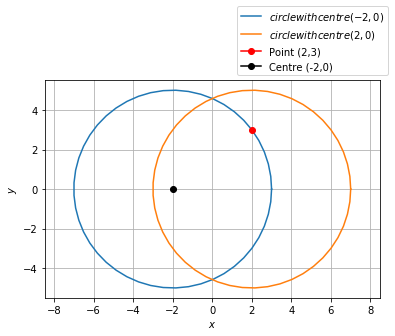
\includegraphics[width=\columnwidth]{./solutions/2/assignment5.png}
    \caption{Circle of radius 5 centre lies on x-axis and passing through the point(2,3)}
    \label{Fig :1solutions/2/}
\end{figure}

qFrom the above figure \ref{Fig :1solutions/2/} it is clear that circle with centre $\vec{c}$=$\myvec{-2\\0}$ passes through the point $\vec{x_1}$

Desired equation of circle is given by  ,
\begin{align}
        c&=\myvec{-2 \\ 0}\\
        f&=-21
\end{align}

